\documentclass[cmbright]{staauth}

\usepackage{amssymb, amsmath, latexsym, array, morefloats, epsfig, rotating, graphicx}
\usepackage{subfigure, url, mathtools, enumerate, wasysym, threeparttable, lscape}
\usepackage{natbib,color}
\usepackage{bm, bbm,epstopdf}
\usepackage{tikz}
\usepackage{xr, zref, hyperref}

\usepackage{bibentry}

\numberwithin{table}{section}

% if variable blind is undefined, assume it is 0
\makeatletter
\@ifundefined{blind}{\def\blind{0}}{}
\makeatother

% if not blinded, reference unblinded paper
\if0\blind
{
  \externaldocument{psokriging}
}\fi

% if blinded, reference blinded paper
\if1\blind
{
  \externaldocument{psokrigingblind}
}\fi


%%%%%%%%%%%%%%%%%%%%%%%%%%%%%%%%%%%%%
\begin{document}
\if0\blind
{
  \runninghead{M Simpson}{AT-PSO for Spatial Design Supporting Material}
  \title{Supporting Web Material: Adaptively-Tuned Particle Swarm Optimization with Application to Spatial Design}
  \author{Matthew Simpson\affil{a}\corrauth, Christopher K. Wikle\affil{a}, Scott H. Holan\affil{a,b}}
  \address{\affilnum{a}Department of Statistics, University of Missouri, 146 Middlebush Hall, Columbia, MO 65211-6100\\
\affilnum{b}U.S. Census Bureau, 4600 Silver Hill Road, Washington, D.C. 20233-9100}
  \corremail{themattsimpson@gmail.com}
  \received{}
  \accepted{}
}\fi

\if1\blind
{
  \runninghead{}{AT-PSO for Spatial Design Supporting Material}
  \title{Supporting Web Material: Adaptively-Tuned Particle Swarm Optimization with Application to Spatial Design}
  \author{}
  \address{}
  \corremail{}
  \received{}
  \accepted{}
}\fi

\maketitle

\appendix
\renewcommand*{\thesection}{S\arabic{section}}
\renewcommand*{\theequation}{S.\arabic{equation}}

\section{PSO and BBPSO details}\label{app:psodetail}

In Section~\ref{sec:pso} we reviewed PSO and BBPSO, and introduced our adaptively tuned variants of both. Here we describe in detail several modifications to both PSO and BBPSO. Most of these are so-called standard modifications from \cite{clerc2011spso}.

\subsection{PSO}\label{subapp:pso}
The standard PSO algorithm is given by \eqref{eq:pso} in the main text. We consider several additions and modifications to this algorithm below. Each of these modifications is combined with adaptively tuned inertia as in \eqref{eq:atpso} to create the AT-PSO algorithms we employ.

\subsubsection{Initialization:}
To initialize the swarm, the number of particles, their initial locations, and their initial velocities have to be chosen. \cite{clerc2011spso} suggests making the swarm size a function of the dimension of the search space, but notes that this is known to be hard to do well and suggests a default swarm size of 40. We use this latter suggestion. We assume the search space is a $D$-dimensional hypercube given by $\bigtimes_{j=1}^D[min_j, max_j]$. Then each particle's initial location is randomly generated uniformly on the cube; i.e., $\theta_{ij}(0)\stackrel{ind}{\sim}U(min_j, max_j)$ for $i=1,2,\dots,n$ and $j=1,2,\dots,D$. Each particle's velocity is initialized based on its location via  $v_{ij}(0)\stackrel{ind}{\sim}U(min_j - x_{ij}(0), max_j - x_{ij}(0))$ for $i=1,2,\dots,n$ and $j=1,2,\dots,D$.

In Section~\ref{sec:houston} each design point is constrained to be in Harris County, TX, which is not a rectangle. We initialize the swarm by placing initial design points on the smallest rectangle containing Harris County. Design points outside of Harris County will quickly move back into the county due to the confinement strategy discussed next.

\subsubsection{Confinement:}
Even though the initialization of the swarm is confined to a hypercube, nothing prevents any given particle from leaving the search space. There are a number of things that can be done in order to address this problem and each has advantages and disadvantages depending on the situation. We focus on two approaches. One is to move any particle that leaves the search space to the nearest point still inside the search space and then adjust its velocity, e.g. \cite{clerc2011spso} suggests that whenever $x_{ij}(k) > max_j$, it should be set to $x_{ij}(k) = max_j$ and similarly when $x_{ij}(k) < min_j$ it should be set to $x_{ij}(k) = min_j$, and in both cases the velocity along that dimension should be reversed and halved, i.e. $v_{ij}(k) = -0.5 v_{ij}(k)$. This causes particles to bounce off the boundary and move back toward the middle of the search space. This is the default strategy we use. This strategy can also be used for more complex search spaces, and in Section~\ref{sec:houston} when a particle leaves Harris County, we move it back to the nearest point in the county and reset the particle's velocity as in the previous paragraph. To move the particle we use the \verb0gNearestPoint0 function from the \verb0rgeos0 \verb0R0 package \citep{rgeos2016, R2016}.

\subsubsection{Redraw Neighborhoods:}
In Section~\ref{sec:pso} we briefly described a variant of the stochastic star neighborhood which we use. This neighborhood is stochastic, meaning that each particle's neighbors are randomly drawn when the algorithm is initialized. After an iteration in which the best known value of the objective function is unchanged, each particle's neighbors are randomly redrawn according to the same distribution.

\subsubsection{Asynchronous Updates:}
The way we defined PSO in \eqref{eq:pso} each particle can update simultaneously. This means that the algorithm is parallelizable, which is a major advantage for implementation on modern GPUs. However, asynchronously updating the particles typically results in faster converging algorithms when it is computationally feasible. In an asynchronous update from period $k$ to $k+1$, particle $i$ recognizes that particle $i-1$ has already updated its personal best location to $\bm{p}_{i-1}(k+1)$ by the time it is $i$'s turn to update. So $i$ computes its group best location taking this into account. This causes particle $i=1$ to behave differently from particle $i=n$ since particle $n$ always has better information in order to perform its update, so every iteration the particles are randomly reordered. More formally, before iteration $k+1$ sample $o_1(k+1), o_2(k+1), \dots, o_{n}(k+1)$ from $\{1,2,\dots,n\}$ without replacement. Then the particles update starting with $o_1(k+1)$, $o_2(k+1)$, etc., so that $o_j(k+1)$ is the $j$th particle to be updated in period $k+1$. Then the group best update becomes $\bm{g}_{o_i}(k+1) = \arg\min_{\{\bm{p}_{o_j}(k+1)|j\in\mathcal{N}_i\}}Q(\bm{p}_j(k_j^*))$ where $k^*_j=k+1$ if $j<i$ and $k$ otherwise. We asynchronously update in all of our algorithms.

\subsubsection{Coordinate Free Velocity Updates:}
The standard velocity update in \eqref{eq:pso} is well known to bias the algorithm toward locations near the coordinate axes and especially the origin \citep{monson2005exposing,spears2010biases}. In general we may not know if the true optimum is near an axis, so this behavior is undesirable. There are several alternative velocity updates available; e.g., see \cite{monson2005exposing}. We use the coordinate free (CF) update suggested by \cite{clerc2011spso}. First define the center of gravity for particle $i$ to be $\bm{C}_i(k) = \bm{\theta}_i(k) + \phi_1\{\bm{p}_i(k) - \bm{\theta}_i(k)\}/3 + \phi_2\{\bm{g}_i(k) - \bm{\theta}_i(k)\}/3$. Let $\mathcal{H}_i(k)$ denote the hypersphere centered at $\bm{C}_i(k)$ with radius $||\bm{C}_i(k) - \bm{\theta}_i(k)||$ where $||\cdot||$ denotes Euclidean distance. Then a new point $\bm{\theta}_i'(k)$ is drawn randomly from $\mathcal{H}_i(k)$ by sampling a direction and a radius, each uniformly. This is \emph{not} the same as drawing uniformly over $\mathcal{H}_i(k)$ and in fact favors points near the center. Then the CF velocity update is given by $\bm{v}_i(k+1) = \omega \bm{v}_i(k) + \bm{x}_i'(k)$. We use both the standard and CF velocity updates in our algorithms. The standard PSO algorithm with each feature in this subsection including the CF velocity update is what \cite{clerc2011spso} calls SPSO 2011.

\subsubsection{When Personal Best Equals the Group Best:}
When a particle's personal best and group best locations coincide, it is often advantageous to allow the particle to explore more than usual. In the standard velocity update we do this by removing the social term so that $\bm{v}_i(k+1) = \omega \bm{v}_i(k) + \phi_1 \bm{r}_{1i}(k)\circ\{\bm{p}_i(k) - \bm{\theta}_i(k)\}$. In the CF velocity update we change the center of gravity to ignore the social term so that $\bm{C}_i(k) = \bm{\theta}_i(k) + \phi_2\{\bm{p}_i(k) - \bm{\theta}_i(k)\}/2$.

\subsection{BBPSO}\label{subapp:bbpso}
The standard BBPSO algorithm was introduced by \cite{kennedy2003bare} and updates from $t$ to $t+1$ via \eqref{eq:bbpso}. We use each of the features in Section~\ref{subapp:pso} in our BBPSO algorithms, though some of them need to be modified for the BBPSO setting. We list them below along with another modification of BBPSO which we employ. Each of these modifications are combined with adaptively tuning a scale parameter as in  \eqref{eq:at-bbpso} to create our AT-BBPSO algorithms.

\subsubsection{BBPSOxp:}
A commonly used variant of BBPSO, also introduced by \cite{kennedy2003bare}, is called BBPSOxp. In this variant, each coordinate of each particle has a 50\% chance of updating according to \eqref{eq:bbpso} and a 50\% chance of moving directly to that particle's personal best location on that coordinate. In other words
\begin{align}\label{eq:bbpsoxp}
\theta_{ij}(k+1) = \begin{cases} N\left\{\frac{p_{ij}(k) + g_{ij}(k)}{2}, h^2_{ij}(k)\right\} & \mbox{with probability }0.5\\
p_{ij}(k) &\mbox{otherwise,}\end{cases}
\end{align}
where $h_{ij}(k) = |p_{ij}(k) - g_{ij}(k)|$. We use both xp and non-xp versions of our BBPSO algorithms.

\subsubsection{CF BBPSO:}
BBPSO's update also depends on the coordinate system since each coordinate of $\bm{\theta}$ gets a different standard deviation. We employ BBPSO algorithms using the default standard deviation, but also using a coordinate free standard deviation given by $h_{ij}(k) = ||\bm{p}_i(k) - \bm{g}_i(k)||$.

\subsubsection{When Personal Best Equals The Group Best in BBPSO:}
A downside of both BBPSO and BBPSOxp is that any particle whose personal best is currently its group best location does not move due to the definition of the standard deviation term. Several methods have been proposed to overcome this; e.g. see \cite{hsieh2010modified} and \cite{zhang2011novel}. \cite{zhang2011novel} propose using mutation and crossover operations for the group best particle. To do this, each group best particle randomly selects three other distinct particles from the entire swarm, $i_1$, $i_2$, and $i_3$, and updates according to
\begin{align}\label{eq:bbpsomc}
\theta_{ij}(k+1) = p_{i_1j}(k) + 0.5\{p_{i_2j}(k) - p_{i_3j}(k)\}.
\end{align}
This combines easily with BBPSOxp to update each coordinate of each particle with $h_{ij}(k)=0$ according to \eqref{eq:bbpsomc} and the rest according to \eqref{eq:bbpsoxp}.

\section{Tables for Comparing PSO and BBPSO algorithms}\label{app:psotabs}

Tables~\ref{tab:psosim1}--\ref{tab:psosim6} contain the simulation results for Objective Functions 1-6 respectively (OF1, OF2, etc.). We use several measures to quantify how well each algorithm finds the global minimum. First, each table includes the mean and standard deviation of the absolute difference between the true global minimum and the algorithm's estimated global minimum across all 40 replications, denoted by Mean and SD. Second, each table includes a convergence criterion --- the proportion of the replications that came within $0.01$ of the true global minimum, denoted by $\widehat{P}$. Finally, $\widehat{K}$ denotes the median number of iterations until the algorithm reaches the convergence criterion; $\widehat{K} > 1000$ indicates that the algorithm did not converge in the allotted 1,000 iterations in at least of $50\%$ of replications. Mean, $\widehat{P}$, and $\widehat{K}$ can be thought of as how close on average the algorithm gets to the global minimum, what proportion of the time it converges, and long it takes to converge respectively. Values for the Mean and SD that are greater than 10,000 are omitted for the sake of readable tables. See Section~\ref{sec:psocompare} (main text) for discussion of these tables.


% latex table generated in R 3.3.1 by xtable 1.8-2 package
% Thu Oct 27 15:18:15 2016
\begin{table}[ht]
\centering
\begingroup\scriptsize
\begin{tabular}{l|rrrr|rrrr|rrrr}
\multicolumn{1}{l}{\begin{tabular}{lr} OF1; & Nbhd: \end{tabular}} & \multicolumn{4}{c}{Global} & \multicolumn{4}{c}{SS3} & \multicolumn{4}{c}{SS1} \\
  \hline
Algorithm & Mean & SD & $\widehat{P}$ & $\widehat{K}$ & Mean & SD & $\widehat{P}$ & $\widehat{K}$ & Mean & SD & $\widehat{P}$ & $\widehat{K}$ \\
  \hline
PSO1 & 0.00 & 0.00 & 1.00 & 205.5 & 0.00 & 0.00 & 1.00 & 358.5 & 384.26 & 891.68 & 0.32 & $> 1000$ \\
  PSO2 & 0.00 & 0.00 & 1.00 & 113 & 0.00 & 0.00 & 1.00 & 200.5 & 724.66 & 1160.10 & 0.20 & $> 1000$ \\
  PSO1-CF & 173.52 & 201.37 & 0.00 & $> 1000$ & 174.60 & 139.70 & 0.00 & $> 1000$ & 1633.30 & 975.59 & 0.00 & $> 1000$ \\
  PSO2-CF & 164.60 & 117.21 & 0.00 & $> 1000$ & 122.56 & 97.48 & 0.00 & $> 1000$ & 1956.30 & 1074.90 & 0.00 & $> 1000$ \\
   \hline
DI-PSO1 & 0.00 & 0.00 & 1.00 & 214 & 0.00 & 0.00 & 1.00 & 265.5 & 1467.50 & 1543.60 & 0.00 & $> 1000$ \\
  DI-PSO2 & 0.00 & 0.00 & 1.00 & 187 & 0.00 & 0.00 & 1.00 & 233.5 & 1641.30 & 1566.30 & 0.00 & $> 1000$ \\
  DI-PSO1-CF & 1709.90 & 897.14 & 0.00 & $> 1000$ & 694.98 & 346.65 & 0.00 & $> 1000$ & 2418.30 & 1140.10 & 0.00 & $> 1000$ \\
  DI-PSO2-CF & 1535.30 & 848.11 & 0.00 & $> 1000$ & 790.97 & 429.16 & 0.00 & $> 1000$ & 2435.10 & 1173.80 & 0.00 & $> 1000$ \\
   \hline
AT1-PSO1 & 0.00 & 0.00 & 1.00 & 186 & 0.00 & 0.00 & 1.00 & 263 & 1962.50 & 1777.20 & 0.00 & $> 1000$ \\
  AT1-PSO2 & 0.00 & 0.00 & 1.00 & 183 & 0.00 & 0.00 & 1.00 & 247 & 932.07 & 1118.20 & 0.00 & $> 1000$ \\
  AT1-PSO1-CF & 329.08 & 260.13 & 0.00 & $> 1000$ & 294.80 & 166.07 & 0.00 & $> 1000$ & 2489.30 & 1040.10 & 0.00 & $> 1000$ \\
  AT1-PSO2-CF & 342.09 & 293.48 & 0.00 & $> 1000$ & 268.43 & 181.01 & 0.00 & $> 1000$ & 2096.10 & 1131.30 & 0.00 & $> 1000$ \\
   \hline
AT2-PSO1 & 0.00 & 0.00 & 1.00 & 112 & 0.00 & 0.00 & 1.00 & 154 & 232.14 & 205.78 & 0.00 & $> 1000$ \\
  AT2-PSO2 & 0.00 & 0.00 & 1.00 & 117 & 0.00 & 0.00 & 1.00 & 150.5 & 127.58 & 164.99 & 0.00 & $> 1000$ \\
  AT2-PSO1-CF & 165.98 & 133.79 & 0.00 & $> 1000$ & 196.39 & 130.15 & 0.00 & $> 1000$ & 1550.60 & 696.54 & 0.00 & $> 1000$ \\
  AT2-PSO2-CF & 118.22 & 77.93 & 0.00 & $> 1000$ & 160.47 & 118.92 & 0.00 & $> 1000$ & 1453.20 & 922.27 & 0.00 & $> 1000$ \\
   \hline
AT1-BBPSO & 0.00 & 0.00 & 1.00 & 740 & 0.00 & 0.00 & 1.00 & 756 & 0.00 & 0.00 & 1.00 & 679.5 \\
  AT1-BBPSOxp & 0.00 & 0.00 & 1.00 & 822.5 & 0.00 & 0.00 & 1.00 & 831 & 0.00 & 0.00 & 1.00 & 694 \\
  AT1-BBPSO-CF & 0.00 & 0.00 & 1.00 & 637 & 0.00 & 0.00 & 1.00 & 642 & 0.00 & 0.00 & 1.00 & 572.5 \\
  AT1-BBPSOxp-CF & 0.00 & 0.00 & 1.00 & 724.5 & 0.00 & 0.00 & 1.00 & 717 & 0.00 & 0.00 & 1.00 & 607.5 \\
   \hline
AT2-BBPSO & 0.00 & 0.00 & 1.00 & 445.5 & 0.00 & 0.00 & 1.00 & 465 & 0.00 & 0.00 & 1.00 & 451 \\
  AT2-BBPSOxp & 0.00 & 0.00 & 1.00 & 501 & 0.00 & 0.00 & 1.00 & 511 & 0.00 & 0.00 & 1.00 & 479 \\
  AT2-BBPSO-CF & 0.00 & 0.00 & 1.00 & 386.5 & 0.00 & 0.00 & 1.00 & 404.5 & 0.00 & 0.00 & 1.00 & 392 \\
  AT2-BBPSOxp-CF & 0.00 & 0.00 & 1.00 & 436.5 & 0.00 & 0.00 & 1.00 & 458 & 0.00 & 0.00 & 1.00 & 420 \\
   \hline
\end{tabular}
\endgroup
\caption{Simulation results for OF1. Each algorithm was run for 1,000 iterations over 40 replications. Mean and SD denote the mean and standard deviation of minimum objective function values found over all replications, while $\widehat{P}$ denotes the proportion of all replications that came within $0.01$ of the true global minimum (equal to zero), and $\widehat{K}$ denotes the median number of iterations until the algorithm came within $0.01$ of the global minimum. Values for the Mean and SD that are greater than 10,000 are omitted.}
\label{tab:psosim1}
\end{table}
% latex table generated in R 3.3.1 by xtable 1.8-2 package
% Thu Oct 27 15:18:15 2016
\begin{table}[ht]
\centering
\begingroup\scriptsize
\begin{tabular}{l|rrrr|rrrr|rrrr}
\multicolumn{1}{l}{\begin{tabular}{lr} OF2; & Nbhd: \end{tabular}} & \multicolumn{4}{c}{Global} & \multicolumn{4}{c}{SS3} & \multicolumn{4}{c}{SS1} \\
  \hline
Algorithm & Mean & SD & $\widehat{P}$ & $\widehat{K}$ & Mean & SD & $\widehat{P}$ & $\widehat{K}$ & Mean & SD & $\widehat{P}$ & $\widehat{K}$ \\
  \hline
PSO1 & 0.00 & 0.00 & 0.92 & 882.5 & 42.08 & 41.70 & 0.00 & $> 1000$ & 3121.10 & 1900.60 & 0.00 & $> 1000$ \\
  PSO2 & 0.00 & 0.00 & 1.00 & 455 & 0.05 & 0.09 & 0.28 & $> 1000$ & 2128.20 & 2264.80 & 0.00 & $> 1000$ \\
  PSO1-CF & 1198.70 & 727.12 & 0.00 & $> 1000$ & 718.76 & 477.04 & 0.00 & $> 1000$ & 3467.90 & 1973.20 & 0.00 & $> 1000$ \\
  PSO2-CF & 892.45 & 593.77 & 0.00 & $> 1000$ & 639.33 & 342.00 & 0.00 & $> 1000$ & 2966.50 & 1426.90 & 0.00 & $> 1000$ \\
   \hline
DI-PSO1 & 52.59 & 108.12 & 0.00 & $> 1000$ & 225.76 & 210.47 & 0.00 & $> 1000$ & 5494.70 & 2604.70 & 0.00 & $> 1000$ \\
  DI-PSO2 & 151.31 & 169.29 & 0.00 & $> 1000$ & 516.50 & 282.07 & 0.00 & $> 1000$ & 4323.90 & 1872.50 & 0.00 & $> 1000$ \\
  DI-PSO1-CF & 3793.40 & 1717.40 & 0.00 & $> 1000$ & 1401.90 & 678.72 & 0.00 & $> 1000$ & 4510.60 & 2058.90 & 0.00 & $> 1000$ \\
  DI-PSO2-CF & 3873.30 & 1935.70 & 0.00 & $> 1000$ & 1566.30 & 733.85 & 0.00 & $> 1000$ & 3637.10 & 1528.20 & 0.00 & $> 1000$ \\
   \hline
AT1-PSO1 & 0.00 & 0.00 & 1.00 & 478.5 & 0.08 & 0.18 & 0.25 & $> 1000$ & 7808.60 & 2929.70 & 0.00 & $> 1000$ \\
  AT1-PSO2 & 0.00 & 0.00 & 1.00 & 481.5 & 0.01 & 0.01 & 0.85 & 924 & 4071.70 & 1647.50 & 0.00 & $> 1000$ \\
  AT1-PSO1-CF & 1424.90 & 620.02 & 0.00 & $> 1000$ & 1021.10 & 509.66 & 0.00 & $> 1000$ & 2910.80 & 1528.70 & 0.00 & $> 1000$ \\
  AT1-PSO2-CF & 1517.60 & 1070.00 & 0.00 & $> 1000$ & 883.77 & 458.02 & 0.00 & $> 1000$ & 2480.30 & 1419.50 & 0.00 & $> 1000$ \\
   \hline
AT2-PSO1 & 91.83 & 356.78 & 0.10 & $> 1000$ & 0.40 & 0.85 & 0.12 & $> 1000$ & 4323.20 & 1925.80 & 0.00 & $> 1000$ \\
  AT2-PSO2 & 5.98 & 20.86 & 0.52 & 979 & 0.23 & 1.24 & 0.60 & 965.5 & 2122.30 & 1402.00 & 0.00 & $> 1000$ \\
  AT2-PSO1-CF & 1358.10 & 766.94 & 0.00 & $> 1000$ & 969.11 & 476.07 & 0.00 & $> 1000$ & 2737.70 & 1082.90 & 0.00 & $> 1000$ \\
  AT2-PSO2-CF & 1078.80 & 640.14 & 0.00 & $> 1000$ & 878.00 & 410.46 & 0.00 & $> 1000$ & 2342.40 & 1427.20 & 0.00 & $> 1000$ \\
   \hline
AT1-BBPSO & 0.06 & 0.03 & 0.00 & $> 1000$ & 0.01 & 0.01 & 0.62 & 989 & 0.00 & 0.00 & 0.90 & 916.5 \\
  AT1-BBPSOxp & 0.67 & 0.41 & 0.00 & $> 1000$ & 0.02 & 0.01 & 0.15 & $> 1000$ & 0.01 & 0.00 & 0.85 & 944 \\
  AT1-BBPSO-CF & 0.03 & 0.01 & 0.05 & $> 1000$ & 0.00 & 0.00 & 0.97 & 916 & 0.00 & 0.00 & 1.00 & 819.5 \\
  AT1-BBPSOxp-CF & 0.35 & 0.22 & 0.00 & $> 1000$ & 0.01 & 0.01 & 0.72 & 972 & 0.00 & 0.00 & 1.00 & 873.5 \\
   \hline
AT2-BBPSO & 0.00 & 0.00 & 1.00 & 852 & 0.00 & 0.00 & 0.92 & 846.5 & 0.00 & 0.00 & 1.00 & 660 \\
  AT2-BBPSOxp & 0.45 & 0.63 & 0.00 & $> 1000$ & 0.05 & 0.13 & 0.50 & 972 & 0.00 & 0.00 & 1.00 & 718 \\
  AT2-BBPSO-CF & 0.00 & 0.00 & 1.00 & 821 & 0.01 & 0.02 & 0.92 & 825 & 0.00 & 0.00 & 1.00 & 636.5 \\
  AT2-BBPSOxp-CF & 0.24 & 0.20 & 0.00 & $> 1000$ & 0.04 & 0.08 & 0.52 & 962 & 0.00 & 0.00 & 1.00 & 682 \\
   \hline
\end{tabular}
\endgroup
\caption{Simulation results for OF2. Each algorithm was run for 1,000 iterations over 40 replications. Mean and SD denote the mean and standard deviation of minimum objective function values found over all replications, while $\widehat{P}$ denotes the proportion of all replications that came within $0.01$ of the true global minimum (equal to zero), and $\widehat{K}$ denotes the median number of iterations until the algorithm came within $0.01$ of the global minimum. Values for the Mean and SD that are greater than 10,000 are omitted.}
\label{tab:psosim2}
\end{table}
% latex table generated in R 3.3.1 by xtable 1.8-2 package
% Thu Oct 27 15:18:15 2016
\begin{table}[ht]
\centering
\begingroup\scriptsize
\begin{tabular}{l|rrrr|rrrr|rrrr}
\multicolumn{1}{l}{\begin{tabular}{lr} OF3; & Nbhd: \end{tabular}} & \multicolumn{4}{c}{Global} & \multicolumn{4}{c}{SS3} & \multicolumn{4}{c}{SS1} \\
  \hline
Algorithm & Mean & SD & $\widehat{P}$ & $\widehat{K}$ & Mean & SD & $\widehat{P}$ & $\widehat{K}$ & Mean & SD & $\widehat{P}$ & $\widehat{K}$ \\
  \hline
PSO1 & 51.84 & 81.96 & 0.00 & $> 1000$ & 32.87 & 35.51 & 0.00 & $> 1000$ &  &  & 0.00 & $> 1000$ \\
  PSO2 & 24.09 & 40.64 & 0.00 & $> 1000$ & 34.97 & 56.51 & 0.00 & $> 1000$ &  &  & 0.00 & $> 1000$ \\
  PSO1-CF &  &  & 0.00 & $> 1000$ &  &  & 0.00 & $> 1000$ &  &  & 0.00 & $> 1000$ \\
  PSO2-CF &  &  & 0.00 & $> 1000$ &  &  & 0.00 & $> 1000$ &  &  & 0.00 & $> 1000$ \\
   \hline
DI-PSO1 & 73.91 & 118.06 & 0.00 & $> 1000$ & 138.79 & 237.03 & 0.00 & $> 1000$ &  &  & 0.00 & $> 1000$ \\
  DI-PSO2 & 73.15 & 101.70 & 0.00 & $> 1000$ & 285.84 & 515.43 & 0.00 & $> 1000$ &  &  & 0.00 & $> 1000$ \\
  DI-PSO1-CF &  &  & 0.00 & $> 1000$ &  &  & 0.00 & $> 1000$ &  &  & 0.00 & $> 1000$ \\
  DI-PSO2-CF &  &  & 0.00 & $> 1000$ &  &  & 0.00 & $> 1000$ &  &  & 0.00 & $> 1000$ \\
   \hline
AT1-PSO1 & 42.13 & 62.63 & 0.00 & $> 1000$ & 27.96 & 32.20 & 0.00 & $> 1000$ &  &  & 0.00 & $> 1000$ \\
  AT1-PSO2 & 29.68 & 49.48 & 0.02 & $> 1000$ & 31.32 & 39.42 & 0.00 & $> 1000$ &  &  & 0.00 & $> 1000$ \\
  AT1-PSO1-CF &  &  & 0.00 & $> 1000$ &  &  & 0.00 & $> 1000$ &  &  & 0.00 & $> 1000$ \\
  AT1-PSO2-CF &  &  & 0.00 & $> 1000$ &  &  & 0.00 & $> 1000$ &  &  & 0.00 & $> 1000$ \\
   \hline
AT2-PSO1 & 63.40 & 150.86 & 0.02 & $> 1000$ & 27.31 & 45.22 & 0.00 & $> 1000$ &  &  & 0.00 & $> 1000$ \\
  AT2-PSO2 & 45.50 & 127.02 & 0.00 & $> 1000$ & 21.57 & 33.17 & 0.00 & $> 1000$ &  &  & 0.00 & $> 1000$ \\
  AT2-PSO1-CF &  &  & 0.00 & $> 1000$ &  &  & 0.00 & $> 1000$ &  &  & 0.00 & $> 1000$ \\
  AT2-PSO2-CF &  &  & 0.00 & $> 1000$ &  &  & 0.00 & $> 1000$ &  &  & 0.00 & $> 1000$ \\
   \hline
AT1-BBPSO & 286.56 & 733.87 & 0.00 & $> 1000$ & 163.98 & 568.42 & 0.00 & $> 1000$ & 55.96 & 68.75 & 0.00 & $> 1000$ \\
  AT1-BBPSOxp & 152.06 & 495.54 & 0.00 & $> 1000$ & 53.66 & 40.22 & 0.00 & $> 1000$ & 38.12 & 36.67 & 0.00 & $> 1000$ \\
  AT1-BBPSO-CF & 121.97 & 358.24 & 0.00 & $> 1000$ & 199.26 & 573.65 & 0.00 & $> 1000$ & 36.63 & 52.87 & 0.00 & $> 1000$ \\
  AT1-BBPSOxp-CF & 390.89 & 857.50 & 0.00 & $> 1000$ & 39.49 & 42.56 & 0.00 & $> 1000$ & 31.37 & 35.33 & 0.00 & $> 1000$ \\
   \hline
AT2-BBPSO & 192.88 & 490.38 & 0.00 & $> 1000$ & 63.77 & 83.78 & 0.00 & $> 1000$ & 84.38 & 132.31 & 0.00 & $> 1000$ \\
  AT2-BBPSOxp & 124.92 & 235.06 & 0.00 & $> 1000$ & 41.88 & 46.31 & 0.00 & $> 1000$ & 34.63 & 36.02 & 0.00 & $> 1000$ \\
  AT2-BBPSO-CF & 325.19 & 767.79 & 0.00 & $> 1000$ & 115.76 & 398.59 & 0.00 & $> 1000$ & 71.89 & 121.28 & 0.00 & $> 1000$ \\
  AT2-BBPSOxp-CF & 229.62 & 646.40 & 0.00 & $> 1000$ & 45.22 & 55.65 & 0.00 & $> 1000$ & 37.75 & 59.87 & 0.00 & $> 1000$ \\
   \hline
\end{tabular}
\endgroup
\caption{Simulation results for OF3. Each algorithm was run for 1,000 iterations over 40 replications. Mean and SD denote the mean and standard deviation of minimum objective function values found over all replications, while $\widehat{P}$ denotes the proportion of all replications that came within $0.01$ of the true global minimum (equal to zero), and $\widehat{K}$ denotes the median number of iterations until the algorithm came within $0.01$ of the global minimum. Values for the Mean and SD that are greater than 10,000 are omitted.}
\label{tab:psosim3}
\end{table}
% latex table generated in R 3.3.1 by xtable 1.8-2 package
% Thu Oct 27 15:18:15 2016
\begin{table}[ht]
\centering
\begingroup\scriptsize
\begin{tabular}{l|rrrr|rrrr|rrrr}
\multicolumn{1}{l}{\begin{tabular}{lr} OF4; & Nbhd: \end{tabular}} & \multicolumn{4}{c}{Global} & \multicolumn{4}{c}{SS3} & \multicolumn{4}{c}{SS1} \\
  \hline
Algorithm & Mean & SD & $\widehat{P}$ & $\widehat{K}$ & Mean & SD & $\widehat{P}$ & $\widehat{K}$ & Mean & SD & $\widehat{P}$ & $\widehat{K}$ \\
  \hline
PSO1 & 3.78 & 1.53 & 0.00 & $> 1000$ & 0.90 & 1.12 & 0.47 & $> 1000$ & 411.24 & 913.72 & 0.00 & $> 1000$ \\
  PSO2 & 8.82 & 4.25 & 0.00 & $> 1000$ & 2.62 & 1.62 & 0.07 & $> 1000$ & 814.28 & 1218.90 & 0.00 & $> 1000$ \\
  PSO1-CF & 504.88 & 318.43 & 0.00 & $> 1000$ & 337.63 & 182.82 & 0.00 & $> 1000$ & 1951.90 & 1010.30 & 0.00 & $> 1000$ \\
  PSO2-CF & 337.14 & 160.49 & 0.00 & $> 1000$ & 253.11 & 127.14 & 0.00 & $> 1000$ & 1973.70 & 971.52 & 0.00 & $> 1000$ \\
   \hline
DI-PSO1 & 7.68 & 2.34 & 0.00 & $> 1000$ & 3.02 & 1.76 & 0.07 & $> 1000$ & 1499.60 & 1649.80 & 0.00 & $> 1000$ \\
  DI-PSO2 & 11.15 & 4.86 & 0.00 & $> 1000$ & 4.71 & 2.28 & 0.00 & $> 1000$ & 1497.30 & 1511.10 & 0.00 & $> 1000$ \\
  DI-PSO1-CF & 1796.40 & 910.83 & 0.00 & $> 1000$ & 780.47 & 623.55 & 0.00 & $> 1000$ & 2276.80 & 1045.00 & 0.00 & $> 1000$ \\
  DI-PSO2-CF & 1652.70 & 826.63 & 0.00 & $> 1000$ & 717.85 & 335.94 & 0.00 & $> 1000$ & 2295.10 & 941.03 & 0.00 & $> 1000$ \\
   \hline
AT1-PSO1 & 4.76 & 2.15 & 0.00 & $> 1000$ & 2.16 & 1.76 & 0.17 & $> 1000$ & 1584.60 & 1101.90 & 0.00 & $> 1000$ \\
  AT1-PSO2 & 6.85 & 2.12 & 0.00 & $> 1000$ & 2.43 & 1.49 & 0.05 & $> 1000$ & 772.81 & 909.62 & 0.00 & $> 1000$ \\
  AT1-PSO1-CF & 963.98 & 737.17 & 0.00 & $> 1000$ & 470.14 & 242.39 & 0.00 & $> 1000$ & 2032.40 & 937.66 & 0.00 & $> 1000$ \\
  AT1-PSO2-CF & 721.45 & 403.80 & 0.00 & $> 1000$ & 358.45 & 172.38 & 0.00 & $> 1000$ & 1780.40 & 650.79 & 0.00 & $> 1000$ \\
   \hline
AT2-PSO1 & 7.44 & 3.39 & 0.00 & $> 1000$ & 3.50 & 1.66 & 0.00 & $> 1000$ & 108.91 & 112.21 & 0.00 & $> 1000$ \\
  AT2-PSO2 & 10.01 & 4.71 & 0.00 & $> 1000$ & 5.02 & 2.70 & 0.00 & $> 1000$ & 122.32 & 191.30 & 0.00 & $> 1000$ \\
  AT2-PSO1-CF & 495.75 & 240.51 & 0.00 & $> 1000$ & 454.87 & 259.16 & 0.00 & $> 1000$ & 1355.10 & 663.30 & 0.00 & $> 1000$ \\
  AT2-PSO2-CF & 425.66 & 293.16 & 0.00 & $> 1000$ & 363.88 & 192.89 & 0.00 & $> 1000$ & 1209.60 & 810.10 & 0.00 & $> 1000$ \\
   \hline
AT1-BBPSO & 3.22 & 1.39 & 0.05 & $> 1000$ & 0.46 & 0.53 & 0.30 & $> 1000$ & 1.15 & 1.23 & 0.35 & $> 1000$ \\
  AT1-BBPSOxp & 0.05 & 0.15 & 0.00 & $> 1000$ & 0.03 & 0.01 & 0.00 & $> 1000$ & 0.14 & 0.35 & 0.65 & 974.5 \\
  AT1-BBPSO-CF & 3.59 & 1.63 & 0.00 & $> 1000$ & 0.24 & 0.52 & 0.80 & 898.5 & 1.17 & 1.15 & 0.35 & $> 1000$ \\
  AT1-BBPSOxp-CF & 0.15 & 0.34 & 0.75 & 985 & 0.01 & 0.00 & 0.85 & 973.5 & 0.12 & 0.32 & 0.88 & 865 \\
   \hline
AT2-BBPSO & 4.59 & 1.93 & 0.00 & $> 1000$ & 0.62 & 0.79 & 0.52 & 633.5 & 1.14 & 1.18 & 0.40 & $> 1000$ \\
  AT2-BBPSOxp & 0.17 & 0.43 & 0.85 & 656 & 0.00 & 0.00 & 1.00 & 672 & 0.12 & 0.32 & 0.88 & 633.5 \\
  AT2-BBPSO-CF & 3.54 & 1.85 & 0.00 & $> 1000$ & 0.59 & 0.74 & 0.52 & 583.5 & 1.57 & 1.30 & 0.22 & $> 1000$ \\
  AT2-BBPSOxp-CF & 0.09 & 0.36 & 0.92 & 591.5 & 0.00 & 0.00 & 1.00 & 614 & 0.10 & 0.29 & 0.90 & 598.5 \\
   \hline
\end{tabular}
\endgroup
\caption{Simulation results for OF4. Each algorithm was run for 1,000 iterations over 40 replications. Mean and SD denote the mean and standard deviation of minimum objective function values found over all replications, while $\widehat{P}$ denotes the proportion of all replications that came within $0.01$ of the true global minimum (equal to zero), and $\widehat{K}$ denotes the median number of iterations until the algorithm came within $0.01$ of the global minimum. Values for the Mean and SD that are greater than 10,000 are omitted.}
\label{tab:psosim4}
\end{table}
% latex table generated in R 3.3.1 by xtable 1.8-2 package
% Thu Oct 27 15:18:15 2016
\begin{table}[ht]
\centering
\begingroup\scriptsize
\begin{tabular}{l|rrrr|rrrr|rrrr}
\multicolumn{1}{l}{\begin{tabular}{lr} OF5; & Nbhd: \end{tabular}} & \multicolumn{4}{c}{Global} & \multicolumn{4}{c}{SS3} & \multicolumn{4}{c}{SS1} \\
  \hline
Algorithm & Mean & SD & $\widehat{P}$ & $\widehat{K}$ & Mean & SD & $\widehat{P}$ & $\widehat{K}$ & Mean & SD & $\widehat{P}$ & $\widehat{K}$ \\
  \hline
PSO1 & 0.03 & 0.03 & 0.30 & $> 1000$ & 0.01 & 0.01 & 0.57 & 441 & 0.52 & 0.65 & 0.07 & $> 1000$ \\
  PSO2 & 0.02 & 0.02 & 0.38 & $> 1000$ & 0.01 & 0.01 & 0.60 & 205 & 0.56 & 0.60 & 0.07 & $> 1000$ \\
  PSO1-CF & 0.89 & 0.20 & 0.00 & $> 1000$ & 0.96 & 0.14 & 0.00 & $> 1000$ & 1.45 & 0.28 & 0.00 & $> 1000$ \\
  PSO2-CF & 0.94 & 0.15 & 0.00 & $> 1000$ & 0.99 & 0.09 & 0.00 & $> 1000$ & 1.48 & 0.31 & 0.00 & $> 1000$ \\
   \hline
DI-PSO1 & 0.02 & 0.02 & 0.28 & $> 1000$ & 0.01 & 0.01 & 0.65 & 258.5 & 1.27 & 0.45 & 0.00 & $> 1000$ \\
  DI-PSO2 & 0.02 & 0.03 & 0.38 & $> 1000$ & 0.01 & 0.02 & 0.65 & 239 & 1.36 & 0.42 & 0.00 & $> 1000$ \\
  DI-PSO1-CF & 1.42 & 0.26 & 0.00 & $> 1000$ & 1.16 & 0.08 & 0.00 & $> 1000$ & 1.60 & 0.30 & 0.00 & $> 1000$ \\
  DI-PSO2-CF & 1.33 & 0.18 & 0.00 & $> 1000$ & 1.15 & 0.09 & 0.00 & $> 1000$ & 1.58 & 0.28 & 0.00 & $> 1000$ \\
   \hline
AT1-PSO1 & 0.02 & 0.02 & 0.42 & $> 1000$ & 0.01 & 0.01 & 0.78 & 253 & 1.37 & 0.28 & 0.00 & $> 1000$ \\
  AT1-PSO2 & 0.02 & 0.02 & 0.32 & $> 1000$ & 0.01 & 0.01 & 0.82 & 239.5 & 1.44 & 0.56 & 0.00 & $> 1000$ \\
  AT1-PSO1-CF & 1.09 & 0.22 & 0.00 & $> 1000$ & 1.04 & 0.10 & 0.00 & $> 1000$ & 1.64 & 0.26 & 0.00 & $> 1000$ \\
  AT1-PSO2-CF & 1.03 & 0.21 & 0.00 & $> 1000$ & 1.04 & 0.11 & 0.00 & $> 1000$ & 1.61 & 0.26 & 0.00 & $> 1000$ \\
   \hline
AT2-PSO1 & 0.03 & 0.03 & 0.38 & $> 1000$ & 0.01 & 0.01 & 0.52 & 167 & 0.93 & 0.28 & 0.00 & $> 1000$ \\
  AT2-PSO2 & 0.03 & 0.03 & 0.35 & $> 1000$ & 0.01 & 0.01 & 0.65 & 132.5 & 0.85 & 0.27 & 0.00 & $> 1000$ \\
  AT2-PSO1-CF & 0.97 & 0.25 & 0.00 & $> 1000$ & 1.02 & 0.10 & 0.00 & $> 1000$ & 1.42 & 0.21 & 0.00 & $> 1000$ \\
  AT2-PSO2-CF & 0.91 & 0.19 & 0.00 & $> 1000$ & 0.97 & 0.10 & 0.00 & $> 1000$ & 1.38 & 0.21 & 0.00 & $> 1000$ \\
   \hline
AT1-BBPSO & 0.01 & 0.01 & 0.55 & 875.5 & 0.00 & 0.01 & 0.85 & 555.5 & 0.00 & 0.01 & 0.82 & 535.5 \\
  AT1-BBPSOxp & 0.01 & 0.01 & 0.72 & 631 & 0.00 & 0.00 & 1.00 & 623.5 & 0.00 & 0.00 & 0.95 & 566.5 \\
  AT1-BBPSO-CF & 0.02 & 0.02 & 0.35 & $> 1000$ & 0.00 & 0.01 & 0.85 & 475 & 0.01 & 0.01 & 0.68 & 472 \\
  AT1-BBPSOxp-CF & 0.01 & 0.01 & 0.78 & 518.5 & 0.00 & 0.00 & 1.00 & 549 & 0.00 & 0.00 & 0.97 & 469.5 \\
   \hline
AT2-BBPSO & 0.02 & 0.02 & 0.40 & $> 1000$ & 0.00 & 0.01 & 0.92 & 366.5 & 0.01 & 0.01 & 0.72 & 406.5 \\
  AT2-BBPSOxp & 0.01 & 0.01 & 0.78 & 387 & 0.00 & 0.00 & 0.97 & 400.5 & 0.00 & 0.01 & 0.90 & 380.5 \\
  AT2-BBPSO-CF & 0.01 & 0.02 & 0.52 & 478.5 & 0.00 & 0.01 & 0.82 & 308.5 & 0.00 & 0.01 & 0.78 & 307 \\
  AT2-BBPSOxp-CF & 0.01 & 0.01 & 0.72 & 370.5 & 0.00 & 0.00 & 1.00 & 342.5 & 0.00 & 0.01 & 0.80 & 349 \\
   \hline
\end{tabular}
\endgroup
\caption{Simulation results for OF5. Each algorithm was run for 1,000 iterations over 40 replications. Mean and SD denote the mean and standard deviation of minimum objective function values found over all replications, while $\widehat{P}$ denotes the proportion of all replications that came within $0.01$ of the true global minimum (equal to zero), and $\widehat{K}$ denotes the median number of iterations until the algorithm came within $0.01$ of the global minimum. Values for the Mean and SD that are greater than 10,000 are omitted.}
\label{tab:psosim5}
\end{table}
% latex table generated in R 3.3.1 by xtable 1.8-2 package
% Thu Oct 27 15:18:15 2016
\begin{table}[ht]
\centering
\begingroup\scriptsize
\begin{tabular}{l|rrrr|rrrr|rrrr}
\multicolumn{1}{l}{\begin{tabular}{lr} OF6; & Nbhd: \end{tabular}} & \multicolumn{4}{c}{Global} & \multicolumn{4}{c}{SS3} & \multicolumn{4}{c}{SS1} \\
  \hline
Algorithm & Mean & SD & $\widehat{P}$ & $\widehat{K}$ & Mean & SD & $\widehat{P}$ & $\widehat{K}$ & Mean & SD & $\widehat{P}$ & $\widehat{K}$ \\
  \hline
PSO1 & 20.01 & 0.02 & 0.00 & $> 1000$ & 20.13 & 0.07 & 0.00 & $> 1000$ & 20.26 & 0.10 & 0.00 & $> 1000$ \\
  PSO2 & 20.00 & 0.01 & 0.00 & $> 1000$ & 20.21 & 0.11 & 0.00 & $> 1000$ & 20.37 & 0.13 & 0.00 & $> 1000$ \\
  PSO1-CF & 20.67 & 0.14 & 0.00 & $> 1000$ & 20.59 & 0.11 & 0.00 & $> 1000$ & 20.56 & 0.13 & 0.00 & $> 1000$ \\
  PSO2-CF & 20.68 & 0.19 & 0.00 & $> 1000$ & 20.62 & 0.11 & 0.00 & $> 1000$ & 20.62 & 0.13 & 0.00 & $> 1000$ \\
   \hline
DI-PSO1 & 20.02 & 0.03 & 0.00 & $> 1000$ & 20.06 & 0.04 & 0.00 & $> 1000$ & 20.11 & 0.05 & 0.00 & $> 1000$ \\
  DI-PSO2 & 20.13 & 0.14 & 0.00 & $> 1000$ & 20.18 & 0.11 & 0.00 & $> 1000$ & 20.23 & 0.09 & 0.00 & $> 1000$ \\
  DI-PSO1-CF & 20.43 & 0.11 & 0.00 & $> 1000$ & 20.33 & 0.10 & 0.00 & $> 1000$ & 20.29 & 0.11 & 0.00 & $> 1000$ \\
  DI-PSO2-CF & 20.48 & 0.13 & 0.00 & $> 1000$ & 20.38 & 0.11 & 0.00 & $> 1000$ & 20.32 & 0.11 & 0.00 & $> 1000$ \\
   \hline
AT1-PSO1 & 20.00 & 0.00 & 0.00 & $> 1000$ & 20.01 & 0.01 & 0.00 & $> 1000$ & 20.00 & 0.00 & 0.00 & $> 1000$ \\
  AT1-PSO2 & 20.02 & 0.04 & 0.00 & $> 1000$ & 20.08 & 0.06 & 0.00 & $> 1000$ & 20.00 & 0.00 & 0.00 & $> 1000$ \\
  AT1-PSO1-CF & 20.06 & 0.06 & 0.00 & $> 1000$ & 20.14 & 0.07 & 0.00 & $> 1000$ & 20.00 & 0.00 & 0.00 & $> 1000$ \\
  AT1-PSO2-CF & 20.23 & 0.09 & 0.00 & $> 1000$ & 20.16 & 0.09 & 0.00 & $> 1000$ & 19.68 & 2.06 & 0.00 & $> 1000$ \\
   \hline
AT2-PSO1 & 20.01 & 0.02 & 0.00 & $> 1000$ & 20.07 & 0.05 & 0.00 & $> 1000$ & 20.22 & 0.09 & 0.00 & $> 1000$ \\
  AT2-PSO2 & 20.12 & 0.10 & 0.00 & $> 1000$ & 20.27 & 0.08 & 0.00 & $> 1000$ & 20.33 & 0.11 & 0.00 & $> 1000$ \\
  AT2-PSO1-CF & 20.33 & 0.10 & 0.00 & $> 1000$ & 20.33 & 0.10 & 0.00 & $> 1000$ & 20.32 & 0.11 & 0.00 & $> 1000$ \\
  AT2-PSO2-CF & 20.38 & 0.12 & 0.00 & $> 1000$ & 20.32 & 0.13 & 0.00 & $> 1000$ & 20.32 & 0.11 & 0.00 & $> 1000$ \\
   \hline
AT1-BBPSO & 17.22 & 8.02 & 0.00 & $> 1000$ & 5.23 & 9.13 & 0.00 & $> 1000$ & 18.71 & 6.28 & 0.00 & $> 1000$ \\
  AT1-BBPSOxp & 18.34 & 6.18 & 0.00 & $> 1000$ & 17.58 & 6.79 & 0.00 & $> 1000$ & 20.42 & 0.21 & 0.00 & $> 1000$ \\
  AT1-BBPSO-CF & 15.63 & 9.14 & 0.07 & $> 1000$ & 0.53 & 3.30 & 0.42 & $> 1000$ & 13.68 & 9.62 & 0.22 & $> 1000$ \\
  AT1-BBPSOxp-CF & 14.75 & 9.19 & 0.00 & $> 1000$ & 10.35 & 9.46 & 0.00 & $> 1000$ & 20.40 & 0.33 & 0.00 & $> 1000$ \\
   \hline
AT2-BBPSO & 17.76 & 7.56 & 0.15 & $> 1000$ & 5.95 & 8.70 & 0.65 & 684.5 & 19.04 & 5.54 & 0.07 & $> 1000$ \\
  AT2-BBPSOxp & 18.22 & 6.18 & 0.10 & $> 1000$ & 17.65 & 5.79 & 0.05 & $> 1000$ & 20.17 & 1.84 & 0.00 & $> 1000$ \\
  AT2-BBPSO-CF & 18.33 & 6.76 & 0.07 & $> 1000$ & 2.06 & 6.25 & 0.90 & 628 & 14.47 & 9.01 & 0.22 & $> 1000$ \\
  AT2-BBPSOxp-CF & 14.49 & 9.15 & 0.28 & $> 1000$ & 10.03 & 8.80 & 0.32 & $> 1000$ & 18.77 & 4.41 & 0.00 & $> 1000$ \\
   \hline
\end{tabular}
\endgroup
\caption{Simulation results for OF6. Each algorithm was run for 1,000 iterations over 40 replications. Mean and SD denote the mean and standard deviation of minimum objective function values found over all replications, while $\widehat{P}$ denotes the proportion of all replications that came within $0.01$ of the true global minimum (equal to zero), and $\widehat{K}$ denotes the median number of iterations until the algorithm came within $0.01$ of the global minimum. Values for the Mean and SD that are greater than 10,000 are omitted.}
\label{tab:psosim6}
\end{table}

\bibliographystyle{wb_stat}
\nobibliography{pso}
\end{document}





Tables~\ref{tab:psosim1}-\ref{tab:psosim6} in the supporting materials contain the simulation results for objective functions 1-6 respectively (OF1, OF2, etc.). We highlight only some of the features of these tables here. The first is that the CF versions of the PSO algorithms do much worse than their corresponding non-CF versions. This is unsurprising since non-CF PSO variants tend to be biased toward finding solutions at the origin and along coordinate axes and each of our objective functions were designed to have a global minimum at the origin. However, for BBPSO variants whether the scale parameter update is CF or not often makes little difference. Often the standard PSO algorithm with either parameter setting, PSO1 or PSO2, and either the Global or SS3 neighborhood performs the best or near the best. Since non-CF PSO algorithms are known to be biased toward the origin and since it is unclear if the DI-PSO and AT-PSO variants are biased to a greater, lesser, or the same degree, PSO1 and PSO2 are not good baselines for comparing to AT variants. Instead we focus on the CF versions of all algorithms. The difference between the CF and non-CF version of each algorithm does serve as a possible measure of the origin-seeking bias of the non-CF version of the algorithm, however.

Narrowing in on the CF algorithms, the AT variants of the PSO-CF algorithms are a mixed bag relative to their pure PSO counterparts. Sometimes the AT version performs better, sometimes not, and often they are essentially indistinguishable. Both classes of algorithms tend to perform better than their DI-PSO-CF counterparts, however, and it is clear for all PSO algorithms that the Global and SS3 neighborhoods both tend to be significantly superior than the SS1 neighborhood. The real story, however, is the performance of the AT-BBPSO-CF variants. Typically they are the best performing CF variant, and often they are even competitive with the best non-CF PSO variants. \emph{Which} AT-BBPSO-CF algorithm performs best depends on the situation. For relatively easy problems such as for OF1 and OF2, AT2 tends to be better than AT1, BBPSO tends to be better than BBPSOxp, and the Global or SS1 neighborhoods tend to be the best across all three measures, so AT2-BBPSO-CF with the Global or SS1 neighborhoods appear attractive. For more complex objective functions such as OF4-OF6, any of the AT-BBPSO-CF variants could perform the best, and whether e.g. AT1 or AT2 is better often interacts with whether the BBPSO or BBPSOxp kernel is used. There does not appear to be a hard an fast rule to abide by, so in more complex optimization problems we recommend trying several AT-BBPSO-CF variants, and perhaps even non-CF variants. Our default recommendation is to try AT2-BBPSO-CF with the global neighborhood. In the case where trying multiple algorithms is worthwhile, e.g. for particularly difficult optimization problems, we recommend experimenting with the neighborhood before experimenting with any of the other knobs on these algorithms. Changing the neighborhood often yields the largest differences between algorithms in our simulations, though sometimes changing the kernel (BBPSO vs. BBPSOxp) or $R^*$ (e.g. AT1 vs. AT2) can also sometimes yield large gains.

The DI-PSO and AT-PSO algorithms are similar conceptually, but often yield very different results. DI-PSO deterministically reduces the inertia parameter over time in the same manner given a fixed set of parameter values ($\alpha$ and $\beta$), while AT-PSO dynamically adjusts the inertia parameter to hit a target improvement rate. Figure~\ref{fig:inertia} plots the inertia over time for the DI-PSO algorithm with $\alpha=200$ and $\beta=1$, and observed inertia over time for one replication of the AT2-PSO2-CF algorithm with the SS3 neighborhood for OF1 and one replication for OF6. DI-PSO smoothly decreases its inertia with a slowly decreasing rate, while AT2-PSO2-CF behaves very differently depending on the objective function. For OF1 it drops the inertia to about to about 0.7 then bounces back up to about 0.8 and fluctuates around that point. This is pretty typical behavior for the inertia parameter of AT-PSO --- it tends to bounce around a level which is approximately the average over time of the DI-PSO's inertia, though lower values of $R^*$ will result in higher inertias. In this way, AT-PSO alternates periods of exploration (relatively high inertia) and periods of exploitation (relatively low inertia). The main exception to this pattern is when AT-PSO converges around a local minimum. In this case, inertia plummets to zero as the particles settle down. This is precisely what happens for OF6 in Figure~\ref{fig:inertia}, though in this case the minimum is not global --- Table~\ref{tab:psosim6} indicates the algorithm never converged to the global min. In optimization problems with multiple local optima, both AT-PSO can exhibit this behavior and prematurely converge to a local minima, so they may not be advantageous for those problems. In theory we expect this behavior for AT-BBPSO as well, but as Table~\ref{tab:psosim6} indicates, some variants of the AT-BBPSO algorithms were able to get significantly closer to the global minimum.

\begin{figure}[!ht]
\centering
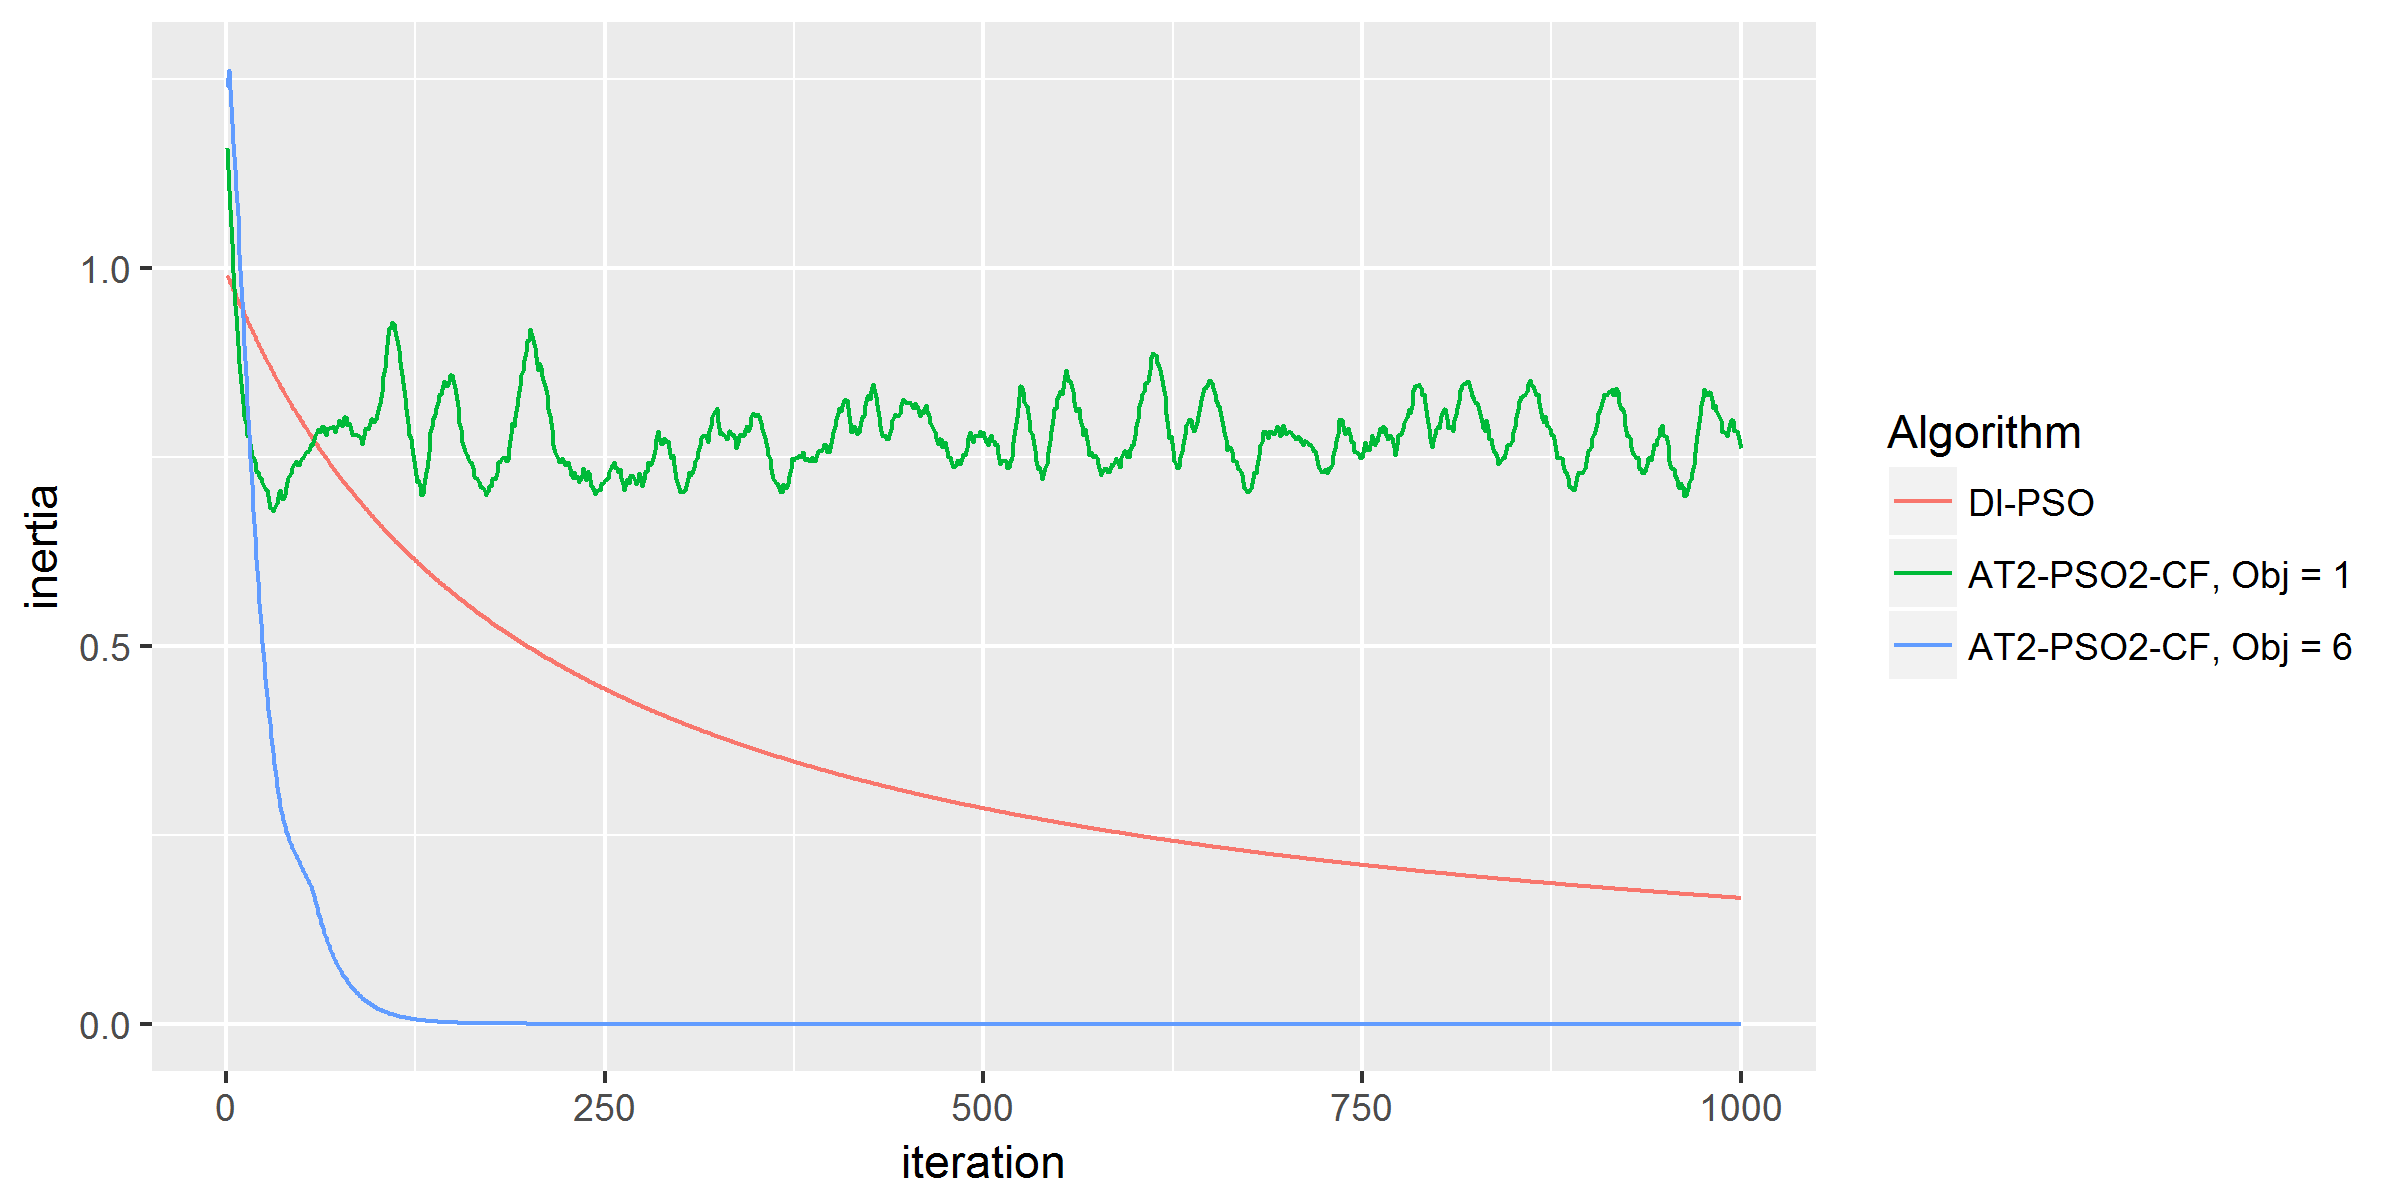
\includegraphics[width=0.95\textwidth]{../code/psosims/inertiaplot.png}
\caption{Inertia over time for the DI-PSO algorithm with $\alpha=200$ and $\beta=1$, and for one replication of the AT-PSO-0.5 algorithm with the SS3 neighborhood for each of OFs 1 and 6.}
\label{fig:inertia}
\end{figure}

Figure~\ref{fig:scale} displays the scale parameter over time for one replication of the AT2-BBPSO-CF algorithm for each of the objective functions we considered with the SS3 neighborhood. Notably, they all result in similar scale parameter dynamics. This holds up remarkably well across replications, BBPSO vs. BBPSOxp, and CF vs. not, such that it may be possible to pick a one-size-fits-all deterministic progression of the scale parameter that matches the algorithm to an AT algorithm with a specific target improvement rate, $R^*$. One key source of variation that is sometimes more pronounced than in Figure~\ref{fig:scale} is that for some objective functions the AT algorithms first increase the scale parameter before following the exponentially decreasing progression. This flexibility to adapt to the objective function may not be worth sacrificing for the one-size-fits all approach. Rather, we highlight this possibility as a possible avenue for further understanding the AT-BBPSO algorithms. 

\begin{figure}[!ht]
\centering
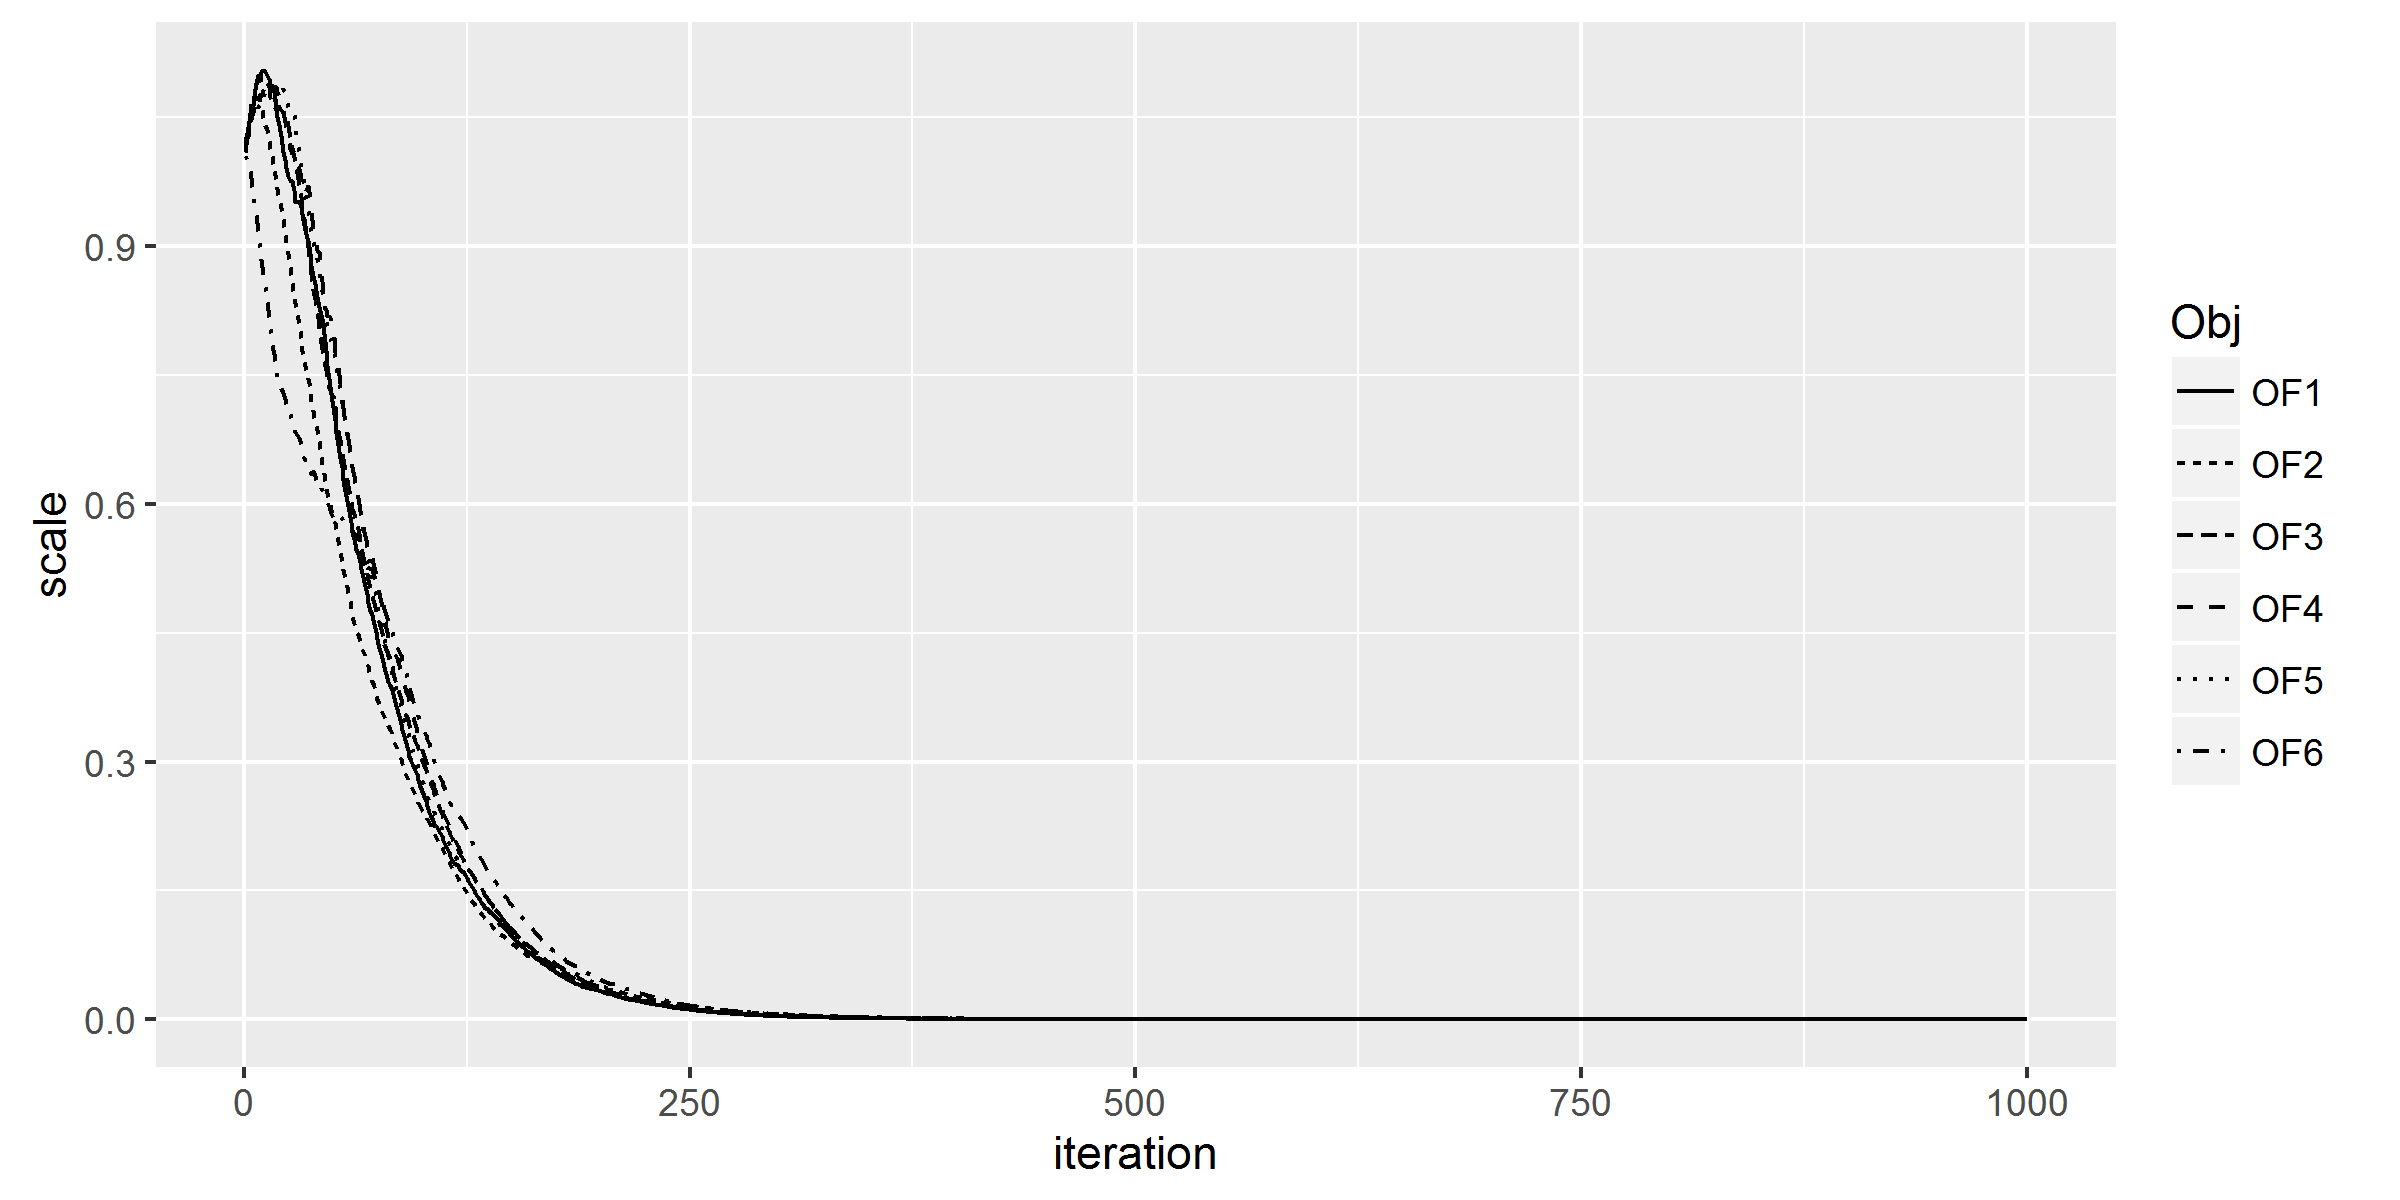
\includegraphics[width=0.95\textwidth]{../code/psosims/scaleplot.png}
\caption{Scale parameter over time for one replication of the the AT2-BBPSO-CF algorithm with the SS3 neighborhood for each of OF1--OF6.}
\label{fig:scale}
\end{figure}

AT-PSO and AT-BBPSO clearly improve on PSO in at least some contexts based on the results of this section. Notably for more difficult problems with, for example, many local optima, the AT algorithms are attractive. In the next section, we turn to applying these algorithms to the practical problem of spatial network design.
